\chapter{Stabilité du génome~: lésions de l'ADN, réparation et recombinaison}\label{ch:b3:dna-repair}

Un après-midi sur une plage dépose quelque cent mille \omterm{def:b3:dna-repair:lesions}{lésions} chimiques
dans l'ADN de chaque cellule de peau exposée au soleil~: des thymines
voisines soudées en dimères par l'ultraviolet, des bases oxydées, des
brins entaillés. Sans le moindre soleil, l'eau tiède de la cellule
arrache chaque jour une dizaine de milliers de purines à leur sucre et
transforme des centaines de cytosines en uracile. Pourtant le taux de
mutation d'une cellule humaine est d'environ un changement pour dix
milliards de paires de bases et par division --- dans un génome de six
milliards, moins d'une mutation nouvelle par division. L'écart entre
les dégâts qu'un génome subit et ceux qu'il garde est comblé par la
réparation~: une douzaine de systèmes enzymatiques patrouillent la
double hélice, reconnaissent ce qui ne devrait pas s'y trouver,
l'excisent et reconstruisent à partir du brin intact et, quand les deux
brins sont rompus, les rejoignent ou recopient le morceau manquant sur
une chromatide sœur. Les enfants privés de l'un de ces systèmes ---
brûlant au premier contact du soleil, ou faisant un cancer du côlon à
trente ans --- montrent ce que ces systèmes valent. Ce chapitre traite
des \omterm{def:b3:dna-repair:lesions}{lésions}, des voies de réparation, de la machinerie de recombinaison
qui répare les pires cassures et que la méiose emprunte, et de la
décision que prend la cellule, quand la réparation échoue, d'arrêter de
se diviser ou de mourir.

\section{Ce qui arrive de fâcheux à l'ADN}

\begin{definition}[Lésions de l'ADN]\label{def:b3:dna-repair:lesions}
\index{lésion de l'ADN}\index{dépurination}\index{désamination}\index{dimère de pyrimidines}\index{cassure double brin}\index{8-oxoguanine}
Une \emph{lésion} est toute altération chimique de l'ADN qui l'écarte
des quatre bases normales correctement appariées sur un squelette
intact. Les lésions spontanées naissent de la chimie de l'eau et du
dioxygène~: la \emph{dépurination}, hydrolyse de la liaison entre une
purine et son sucre, qui laisse un site abasique (environ $10^{4}$ par
cellule et par jour)~; la \emph{désamination}, qui transforme la
cytosine en uracile, la 5-méthylcytosine en thymine et l'adénine en
hypoxanthine (quelques centaines par jour)~; l'\emph{oxydation} par les
espèces réactives de l'oxygène, principalement en \emph{8-oxoguanine},
qui s'apparie aussi volontiers à l'adénine qu'à la cytosine~; et les
\emph{erreurs de réplication}, base mal incorporée ou glissement. Parmi
les lésions d'origine environnementale figurent le \emph{dimère
cyclobutanique de pyrimidines} et le photoproduit 6-4 que l'ultraviolet
forme entre deux pyrimidines voisines~; les bases alkylées dues aux
agents alkylants (l'O$^{6}$-méthylguanine s'apparie à la thymine)~; les
adduits volumineux dus aux hydrocarbures aromatiques et à
l'aflatoxine~; les pontages interbrins dus au cisplatine et aux
moutardes azotées~; et les cassures simple brin et \emph{double brin}
produites par les rayonnements ionisants, soit environ \num{1000}
cassures simple brin et \numrange{30}{40} cassures double brin par
cellule et par gray.
\end{definition}

\begin{proposition}[L'échelle de fidélité]\label{prop:b3:dna-repair:fidelity}
\index{fidélité}\index{relecture}\index{réparation des mésappariements}
La réplication atteint son taux d'erreur d'environ $10^{-10}$ par paire
de bases en trois étapes multiplicatives. La sélection de la base par
la polymérase, sur la géométrie et les liaisons hydrogène, se trompe
environ une fois sur $10^{5}$~; la \emph{relecture} par l'exonucléase
3$'\to$5$'$ de la polymérase, qui excise une base terminale mal
appariée avant l'élongation, en supprime \qty{99}{\%}~; la
\emph{\omterm{prop:b3:dna-repair:fidelity}{réparation des mésappariements}}, qui agit derrière la fourche sur
le brin néoformé, supprime \qty{99.9}{\%} de ce qui reste. Le produit
$10^{-5}\times 10^{-2}\times 10^{-3} = 10^{-10}$ est le taux observé,
et un défaut de l'une ou l'autre correction le multiplie par cent ou
par mille~: de telles cellules sont \emph{mutatrices}.
\end{proposition}

\begin{example}[Lésions contre mutations]\label{ex:b3:dna-repair:numbers}
Une cellule humaine de $6.4\times 10^{9}$ paires de bases qui se divise
une fois par jour accumule de l'ordre de $10^{4}$--$10^{5}$ \omterm{def:b3:dna-repair:lesions}{lésions} par
jour et environ $6.4\times 10^{9}\times 10^{-10} \approx 0.6$ mutation
nouvelle par division~: moins d'une \omterm{def:b3:dna-repair:lesions}{lésion} sur dix mille survit et
devient un changement définitif. Les autres sont réparées avant que la
réplication ne les lise, et c'est le taux de survie jusqu'à la mutation
--- et non le taux de dégâts --- que la sélection a minimisé. La même
arithmétique montre pourquoi le nombre de mutations d'une tumeur ou du
sperme d'un père âgé compte des divisions~: les mutations qu'une
cellule porte sont, au premier ordre, les divisions qu'elle a subies
multipliées par l'erreur par division.
\end{example}

\section{Réparer un brin abîmé}

\begin{definition}[Réparation par excision]\label{def:b3:dna-repair:excision}
\index{réparation par excision de base}\index{réparation par excision de nucléotides}\index{glycosylase}\index{xeroderma pigmentosum}
La plupart des \omterm{def:b3:dna-repair:lesions}{lésions} n'atteignent qu'un brin et sont réparées en
découpant le morceau abîmé et en recopiant l'autre brin. La
\emph{réparation par excision de base} (BER) traite les petites \omterm{def:b3:dna-repair:lesions}{lésions}
qui ne déforment pas l'hélice~: une \emph{ADN-glycosylase} propre à un
type de base fautive (uracile-ADN-glycosylase, glycosylase de la
8-oxoG, et plusieurs autres) bascule la base hors de l'hélice et la
détache de son sucre~; une AP-endonucléase entaille le squelette au
site abasique~; une polymérase (Pol~$\beta$) retire le sucre et insère
un nucléotide~; une ligase scelle. La \emph{réparation par excision de
nucléotides} (NER) traite les \omterm{def:b3:dna-repair:lesions}{lésions} volumineuses qui déforment
l'hélice --- \omterm{def:b3:dna-repair:lesions}{dimères de pyrimidines}, adduits chimiques --- sans
reconnaître la chimie de la \omterm{def:b3:dna-repair:lesions}{lésion} elle-même~: la déformation est
détectée (par XPC qui balaie le génome, ou par une ARN polymérase
bloquée dans la branche couplée à la transcription), l'hélice est
ouverte par les sous-unités hélicases de TFIIH, le dommage est vérifié
(XPA), deux endonucléases (XPF, XPG) coupent le brin lésé à
\numrange{24}{32} nucléotides d'intervalle, l'oligonucléotide est
libéré, et polymérase et ligase comblent la brèche. La perte de l'une
des sept protéines XP cause le \emph{xeroderma pigmentosum}~: extrême
sensibilité au soleil, éphélides, et taux de cancer cutané multiplié
par mille.
\end{definition}

\begin{proof}[Faits expérimentaux]
Cleaver (1968) a cultivé des fibroblastes cutanés de patients atteints
de \omterm{def:b3:dna-repair:excision}{xeroderma pigmentosum}, les a irradiés aux ultraviolets et leur a
donné de la thymidine radioactive hors de la phase~S. Les cellules
normales incorporaient le marqueur en de nombreux petits sites --- la
«~synthèse d'ADN non programmée~» des rustines de réparation --- tandis
que les cellules des patients n'en incorporaient presque pas et
mouraient à des doses que les cellules normales supportaient~: la
maladie est un défaut d'excision des dimères. La fusion de cellules de
deux patients rétablissait souvent la réparation dans l'hybride, chacune
fournissant ce qui manquait à l'autre~; par ce test les patients ont été
répartis en groupes de complémentation A à G, un par gène de la voie,
des années avant le clonage des gènes.
\end{proof}

\begin{omfigure}
\begin{tikzpicture}[every node/.style={font=\scriptsize}, >=stealth]
  % BER column
  \node[font=\small\bfseries] at (2.0,3.2) {Réparation par excision de base};
  \foreach \y/\txt in {2.6/{base lésée (U, 8-oxoG)}, 1.5/{la glycosylase retire la base}, 0.4/{l'AP-endonucléase entaille}, -0.7/{Pol $\beta$ comble un nucléotide, la ligase scelle}} {
    \draw[very thick, omDef] (0.2,\y) -- (3.8,\y); \draw[very thick, omDef] (0.2,\y-0.25) -- (3.8,\y-0.25);
    \node[right, align=left] at (0.2,\y-0.6) {\txt};
  }
  \fill[omThm] (2.0,2.6) circle (0.1);
  \draw[omThm, thick] (1.9,1.5) -- (2.1,1.5);
  \draw[white, very thick] (1.9,0.4) -- (2.1,0.4);
  \fill[omMeth!80!black] (2.0,-0.7) circle (0.1);
  % NER column
  \node[font=\small\bfseries] at (8.0,3.2) {Réparation par excision de nucléotides};
  \foreach \y/\txt in {2.6/{la lésion volumineuse déforme l'hélice~; XPC se fixe}, 1.5/{TFIIH ouvre l'hélice, XPA vérifie}, 0.4/{XPF et XPG coupent à 24--32 nt d'intervalle}, -0.7/{la polymérase comble la brèche, la ligase scelle}} {
    \draw[very thick, omDef] (6.2,\y) -- (9.8,\y); \draw[very thick, omDef] (6.2,\y-0.25) -- (9.8,\y-0.25);
    \node[right, align=left] at (6.2,\y-0.6) {\txt};
  }
  \draw[omThm, very thick] (7.8,2.6) -- (8.2,2.6) -- (8.2,2.75) -- (7.8,2.75) -- cycle;
  \draw[omDef, very thick] (7.2,1.5) .. controls (7.6,1.85) and (8.4,1.85) .. (8.8,1.5); \draw[omThm, very thick] (7.85,1.72) -- (8.15,1.72);
  \draw[very thick, white] (7.0,0.4) -- (9.0,0.4); \draw[omThm, thick, ->] (7.0,0.7) -- (7.0,0.48); \draw[omThm, thick, ->] (9.0,0.7) -- (9.0,0.48);
  \draw[very thick, omMeth!80!black] (7.0,-0.7) -- (9.0,-0.7);
\end{tikzpicture}

{\small Deux voies d'excision. L'excision de base (à gauche) reconnaît
une base fautive précise à l'aide d'une \omterm{def:b3:dna-repair:excision}{glycosylase} dédiée et remplace
un nucléotide. L'excision de nucléotides (à droite) reconnaît la
déformation que cause toute \omterm{def:b3:dna-repair:lesions}{lésion} volumineuse, coupe le brin de part
et d'autre et remplace une rustine d'une trentaine de nucléotides
(vert).}
\end{omfigure}

\begin{definition}[Réparation des mésappariements]\label{def:b3:dna-repair:mmr}
\index{réparation des mésappariements!discrimination des brins}\index{syndrome de Lynch}\index{instabilité des microsatellites}
La \emph{\omterm{prop:b3:dna-repair:fidelity}{réparation des mésappariements}} (MMR) corrige les mauvais
appariements et les petites boucles d'insertion ou de délétion qui
échappent à la relecture. La protéine MutS (MSH2--MSH6 chez l'homme)
reconnaît la déformation d'un mésappariement et, avec MutL
(MLH1--PMS2), autorise une exonucléase à dégrader le brin néosynthétisé
depuis une entaille voisine jusqu'au-delà du mésappariement~; la brèche
est ensuite comblée par une polymérase. La difficulté est la
\emph{discrimination des brins}~: un mésappariement comporte deux bases
et une seule est fautive. Chez \emph{Escherichia coli} le brin neuf est
reconnu parce qu'il n'est pas encore méthylé aux sites GATC, que la
méthylase Dam marque quelques minutes après la synthèse~; MutH entaille
le brin non méthylé. Chez les eucaryotes le brin neuf est reconnu grâce
aux entailles entre fragments d'Okazaki et à l'extrémité 3$'$ libre du
brin continu. La perte de la MMR multiplie par cent ou par mille le
taux de mutation, surtout aux \emph{microsatellites} --- suites d'une
courte répétition où la polymérase glisse --- dont les longueurs
changent d'une cellule à l'autre~: c'est l'\emph{instabilité des
microsatellites}. La perte héritée d'un allèle de la MMR constitue le
\emph{syndrome de Lynch}, avec un cancer colorectal chez quelque
\qty{70}{\%} des porteurs, souvent avant cinquante ans.
\end{definition}

\begin{omfigure}
\begin{tikzpicture}[every node/.style={font=\scriptsize}, >=stealth]
  \draw[very thick, omDef] (0,1.2) -- (9,1.2); \node[left] at (-0.1,1.2) {brin matrice};
  \draw[very thick, gray] (0,0.6) -- (9,0.6); \node[left] at (-0.1,0.6) {brin neuf};
  % methyl groups on template at GATC
  \foreach \x in {1.5,7.5} { \fill[omMeth!80!black] (\x,1.35) circle (0.1); \node[above] at (\x,1.45) {CH$_3$ sur GATC}; }
  \foreach \x in {1.5,7.5} { \draw[omMeth!80!black] (\x,0.45) circle (0.1); }
  \node[below] at (7.5,0.32) {pas encore méthylé};
  % mismatch
  \draw[omThm, very thick] (4.5,1.05) -- (4.5,0.75); \node[omThm, right] at (4.6,0.9) {mésappariement};
  \draw[thick, fill=omExo!35] (4.5,1.9) ellipse (1.0 and 0.3); \node at (4.5,1.9) {MutS/MutL};
  \draw[->, thick] (4.5,1.65) -- (4.5,1.3);
  % MutH nick on new strand at unmethylated GATC
  \draw[omThm, thick, ->] (1.5,-0.55) -- (1.5,0.42); \node[omThm, below] at (1.5,-0.55) {MutH entaille le brin non méthylé};
  % excision arrow
  \draw[->, very thick, omProp] (1.7,-0.1) -- (5.0,-0.1); \node[omProp, below] at (3.95,-0.15) {l'exonucléase dégrade au-delà du mésappariement};
  \node[right] at (5.4,-0.8) {puis Pol III comble la brèche, la ligase scelle};
\end{tikzpicture}

{\small La discrimination des brins dans la réparation bactérienne des
mésappariements. Le brin matrice porte des groupements méthyle à ses
sites GATC~; le brin neuf n'en porte pas encore, et MutH l'entaille
là. La base fautive est donc toujours retirée du brin neuf.}
\end{omfigure}

\begin{method}[Répartir une maladie de la réparation entre des gènes]\label{met:b3:dna-repair:complementation}
\index{test de complémentation}
Pour savoir combien de gènes met en jeu un phénotype récessif, avant
qu'aucun gène ne soit connu~: (1) prendre des lignées cellulaires de
patients non apparentés, chacune mutée dans un gène de la voie~;
(2) fusionner des paires de lignées en cellules hybrides~; (3) tester
la fonction dans l'hybride (ici la synthèse d'ADN non programmée après
ultraviolet)~; (4) si l'hybride répare, les deux patients portent des
mutations dans des gènes \emph{différents} (chacun fournit la protéine
qui manque à l'autre~: ils se \emph{complémentent})~; sinon, dans le
même gène~; (5) répartir les patients en groupes de complémentation ---
un par gène. Le nombre de groupes est un minorant du nombre de gènes.
\end{method}

\section{Réparer un chromosome cassé}

\begin{definition}[Réparation des cassures double brin]\label{def:b3:dna-repair:dsb}
\index{jonction d'extrémités non homologues}\index{recombinaison homologue}\index{Rad51}\index{jonction de Holliday}\index{BRCA}
Une \emph{\omterm{def:b3:dna-repair:lesions}{cassure double brin}} sectionne le chromosome et ne laisse
aucun brin intact à recopier. Deux voies la réparent. La \emph{jonction
d'extrémités non homologues} (NHEJ)~: l'anneau Ku70--Ku80 se fixe sur
chaque extrémité, recrute la kinase DNA-PKcs, des nucléases ébarbent
les extrémités sortantes, et la ligase~IV joint les bouts~; elle
fonctionne à toute phase du cycle et en quelques minutes, mais elle
perd ou ajoute quelques nucléotides à la jonction et peut joindre les
mauvaises extrémités. La \emph{recombinaison homologue} (HR)~: le
complexe MRN et des nucléases résèquent les brins 5$'$ pour laisser de
longues queues 3$'$ simple brin, recouvertes par RPA puis, avec l'aide
de BRCA2, par la recombinase \emph{Rad51}~; le filament de Rad51
cherche un duplex homologue --- la chromatide sœur, en S et en G2 ---
l'envahit, et l'extrémité 3$'$ envahissante amorce une synthèse sur la
copie intacte. Les molécules jointes peuvent être dissoutes après une
courte synthèse (la plupart des réparations mitotiques, sans échange de
l'ADN flanquant) ou mûrir en deux \emph{jonctions de Holliday} à quatre
branches, dont la résolution par des endonucléases donne un produit
avec ou sans crossing-over. La HR est fidèle parce qu'elle recopie une
sœur, mais elle n'est disponible que s'il existe une sœur.
\end{definition}

\begin{omfigure}
\begin{tikzpicture}[every node/.style={font=\scriptsize}, >=stealth]
  % break
  \draw[very thick, omDef] (0,3.2) -- (2.3,3.2); \draw[very thick, omDef] (2.7,3.2) -- (5,3.2);
  \draw[very thick, omDef] (0,3.0) -- (2.3,3.0); \draw[very thick, omDef] (2.7,3.0) -- (5,3.0);
  \node[above] at (2.5,3.3) {cassure double brin};
  % NHEJ left
  \draw[->, thick] (1.2,2.8) -- (-0.5,2.0); \node[left, align=right] at (-0.6,2.4) {toute phase,\\quelques minutes};
  \node[font=\small\bfseries] at (-1.6,1.55) {NHEJ};
  \draw[thick, fill=omExo!35] (-2.6,0.9) ellipse (0.3 and 0.2); \draw[thick, fill=omExo!35] (-0.8,0.9) ellipse (0.3 and 0.2);
  \draw[very thick, omDef] (-3.4,0.9) -- (-2.9,0.9); \draw[very thick, omDef] (-0.5,0.9) -- (0.0,0.9);
  \node[below] at (-1.7,0.7) {Ku se fixe aux deux bouts, ébarbage};
  \draw[->, thick] (-1.7,0.3) -- (-1.7,-0.1);
  \draw[very thick, omDef] (-3.4,-0.4) -- (0.0,-0.4); \draw[omThm, very thick] (-1.85,-0.4) -- (-1.55,-0.4);
  \node[below, align=center] at (-1.7,-0.55) {la ligase IV joint~:\\quelques nucléotides perdus ou ajoutés};
  % HR right
  \draw[->, thick] (3.8,2.8) -- (5.5,2.0); \node[right, align=left] at (5.6,2.4) {S/G2, une sœur\\présente~; quelques heures};
  \node[font=\small\bfseries] at (6.8,1.55) {HR};
  % resected ends
  \draw[very thick, omDef] (4.6,0.9) -- (6.2,0.9); \draw[very thick, omDef] (7.4,0.9) -- (9.0,0.9);
  \draw[very thick, omDef] (4.6,0.7) -- (5.6,0.7); \draw[very thick, omDef] (8.0,0.7) -- (9.0,0.7);
  \foreach \x in {5.7,5.9,6.1} \fill[omProp] (\x,0.9) circle (0.07);
  \node[below] at (6.8,0.55) {résection 5$'$~; Rad51 recouvre les queues 3$'$};
  \draw[->, thick] (6.8,0.15) -- (6.8,-0.25);
  % strand invasion of sister
  \draw[very thick, omMeth!70!black] (4.6,-0.9) -- (9.0,-0.9); \draw[very thick, omMeth!70!black] (4.6,-1.1) -- (9.0,-1.1);
  \draw[very thick, omDef] (4.6,-0.5) -- (5.8,-0.5) .. controls (6.2,-0.5) and (6.3,-0.9) .. (6.6,-0.9) -- (7.6,-0.9);
  \draw[->, omDef, thick] (7.6,-0.9) -- (8.1,-0.9);
  \node[below, align=center] at (6.8,-1.2) {invasion de la sœur (vert), synthèse sur la copie intacte,\\puis dissolution (sans crossing-over) ou jonctions de Holliday};
\end{tikzpicture}

{\small Les deux destins d'une \omterm{def:b3:dna-repair:lesions}{cassure double brin}. À gauche~: la
jonction d'extrémités, rapide et toujours disponible, au prix d'un
petit changement à la jonction. À droite~: la \omterm{def:b3:dna-repair:dsb}{recombinaison homologue},
qui résèque les extrémités, envahit la chromatide sœur avec un filament
de \omterm{def:b3:dna-repair:dsb}{Rad51} et recopie ce qui a été perdu.}
\end{omfigure}

\begin{theorem}[Charge de lésions, vitesse de réparation et fourche]\label{thm:b3:dna-repair:load}
\index{dommages résiduels}\index{voies concurrentes}
Soit des \omterm{def:b3:dna-repair:lesions}{lésions} d'un même type apparaissant à la vitesse constante $D$
par cellule et par heure et retirées par une réparation du premier
ordre de constante $k$ (demi-vie $t_{1/2} = \ln 2/k$). Le nombre de
\omterm{def:b3:dna-repair:lesions}{lésions} $L(t)$ obéit à $\mathrm{d}L/\mathrm{d}t = D - kL$, de sorte
qu'à l'état stationnaire
\[
L^{*} = \frac{D}{k},
\]
et qu'une impulsion de $N$ \omterm{def:b3:dna-repair:lesions}{lésions} délivrée en $t = 0$ en laisse
$N e^{-kT}$ lorsqu'une fourche de réplication arrive au temps $T$. Si
deux voies se disputent la même \omterm{def:b3:dna-repair:lesions}{lésion} avec les constantes $k_{1}$ et
$k_{2}$, chaque \omterm{def:b3:dna-repair:lesions}{lésion} est réparée par la première avec la probabilité
$k_{1}/(k_{1} +
k_{2})$ et la demi-vie globale vaut $\ln 2/(k_{1} + k_{2})$. Le nombre
de \omterm{def:b3:dna-repair:lesions}{lésions} qui atteignent la fourche suit une loi de Poisson de moyenne
$N e^{-kT}$, de sorte que la probabilité qu'aucune n'y parvienne vaut
$\exp(-N e^{-kT})$.
\end{theorem}
\begin{proof}
L'état stationnaire est là où $D = kL$. Pour l'impulsion, $D = 0$ et
l'équation s'intègre en $L = N e^{-kt}$. Avec deux voies, la vitesse de
perte est $(k_{1} + k_{2})L$~; sur un court intervalle une \omterm{def:b3:dna-repair:lesions}{lésion}
donnée est retirée par la voie~1 avec la probabilité
$k_{1}\,\mathrm{d}t$ et par la voie~2 avec $k_{2}\,\mathrm{d}t$, donc
la probabilité conditionnelle que son retrait, lorsqu'il a lieu, soit
le fait de la voie~1 vaut $k_{1}/(k_{1} +
k_{2})$. Des \omterm{def:b3:dna-repair:lesions}{lésions} indépendantes survivant chacune avec la
probabilité $e^{-kT}$ donnent un comptage binomial, poissonnien à la
limite de nombreuses \omterm{def:b3:dna-repair:lesions}{lésions} et d'une faible survie, et la probabilité
poissonnienne de zéro vaut $e^{-\text{moyenne}}$.
\end{proof}

\begin{example}[Pourquoi le xeroderma est une maladie de la fourche]\label{ex:b3:dna-repair:xp}
Une dose de soleil laisse $N = 10^{5}$ \omterm{def:b3:dna-repair:lesions}{dimères de pyrimidines} dans un
kératinocyte. Avec une demi-vie d'excision de nucléotides de \qty{2}{h}
($k =
\qty{0.35}{h^{-1}}$) et une fourche qui arrive au bout de \qty{8}{h},
$N e^{-kT} =
10^{5}\times e^{-2.8} \approx 6000$ dimères sont encore là pour être
recopiés~; avec la réparation quasi nulle d'une cellule XP ($k \approx
\qty{0.01}{h^{-1}}$), il y en a \num{92000}. Chaque dimère rencontré
par la fourche est contourné par une \omterm{def:b3:dna-repair:tls}{synthèse translésionnelle} (plus
bas), infidèle~: la charge de mutations du patient par division est
quinze fois la normale, et les cancers cutanés suivent dès l'enfance.
Le seul remède efficace est de maintenir $N$ petit --- l'évitement
total des ultraviolets.
\end{example}

\begin{omfigure}
\begin{tikzpicture}
\begin{axis}[
  width=0.7\linewidth, height=5.6cm,
  axis x line=bottom, axis y line=left,
  xmin=0, xmax=12, ymin=100, ymax=200000, ymode=log,
  xlabel={heures après l'exposition}, ylabel={dimères par cellule},
  xlabel style={font=\small, at={(axis description cs:0.5,-0.12)}, anchor=north},
  ylabel style={font=\small},
  tick label style={font=\small}, xtick={0,2,4,6,8,10,12},
  clip=false,
]
\addplot[very thick, omDef, domain=0:12, samples=40] {100000*exp(-0.35*x)};
\addplot[very thick, omThm, domain=0:12, samples=40] {100000*exp(-0.01*x)};
\addplot[dashed, gray] coordinates {(8,100) (8,200000)};
\node[font=\scriptsize, anchor=south east, gray] at (axis cs:8,110) {la fourche arrive};
\node[font=\scriptsize, omDef, anchor=north east] at (axis cs:11.5,18000) {normale, $t_{1/2} = \qty{2}{h}$};
\node[font=\scriptsize, omThm, anchor=south west] at (axis cs:2,105000) {xeroderma pigmentosum};
\fill[omDef] (axis cs:8,6070) circle (2pt); \node[font=\scriptsize, omDef, anchor=west] at (axis cs:8.3,6070) {\num{6000}};
\fill[omThm] (axis cs:8,92300) circle (2pt); \node[font=\scriptsize, omThm, anchor=north west] at (axis cs:8.3,80000) {\num{92000}};
\end{axis}
\end{tikzpicture}

{\small Dimères restants après une impulsion de $10^{5}$, en échelle
logarithmique, pour une cellule normale et pour une cellule déficiente
en excision de nucléotides. La fourche, à \qty{8}{h}, rencontre quinze
fois plus de \omterm{def:b3:dna-repair:lesions}{lésions} dans la cellule du patient.}
\end{omfigure}

\begin{proof}[Faits expérimentaux]
Holliday (1964) a proposé la jonction à quatre branches pour expliquer
une énigme de la génétique des champignons~: dans un croisement, une
tétrade de spores montrait parfois une ségrégation $3{:}1$ au lieu du
$2{:}2$ mendélien pour un marqueur, toujours pour des marqueurs proches
d'un crossing-over. Son modèle --- l'échange de brins isolés entre deux
duplex homologues, formant un hétéroduplex que la \omterm{prop:b3:dna-repair:fidelity}{réparation des
mésappariements} «~corrige~» ensuite dans un sens ou dans l'autre
(\emph{conversion génique}) --- expliquait à la fois ces rapports
étranges et leur association au crossing-over. La jonction elle-même a
été vue plus tard au microscope électronique dans des plasmides en
recombinaison et dans la structure de la résolvase RuvC qui s'y fixe.
\end{proof}

\section{Tolérance, alerte et décision d'arrêter}

\begin{definition}[Synthèse translésionnelle]\label{def:b3:dna-repair:tls}
\index{synthèse translésionnelle}\index{polymérase êta}
Quand une fourche rencontre une \omterm{def:b3:dna-repair:lesions}{lésion} qui n'a pas été réparée, la
polymérase réplicative cale. La \emph{synthèse translésionnelle} (TLS)
appelle une polymérase spécialisée, au site actif plus vaste et sans
relecture --- Pol~$\eta$ pour les \omterm{def:b3:dna-repair:lesions}{dimères de pyrimidines}, Pol~$\iota$,
$\kappa$, $\zeta$ et Rev1 pour d'autres \omterm{def:b3:dna-repair:lesions}{lésions} --- qui insère quelques
nucléotides en face de la \omterm{def:b3:dna-repair:lesions}{lésion} puis s'efface. Pol~$\eta$ place deux
adénines en face d'un dimère de thymines, ce qui est généralement
juste~; les autres se trompent souvent. La TLS échange la fidélité
contre la survie de la fourche, et elle est la source de la plupart des
mutations induites par l'ultraviolet. La forme variante du \omterm{def:b3:dna-repair:excision}{xeroderma
pigmentosum} (XP-V) a une excision intacte et manque de Pol~$\eta$~: les
dimères qui échappent à l'excision sont contournés par des polymérases
plus infidèles, et les cancers suivent.
\end{definition}

\begin{proposition}[La réponse SOS bactérienne]\label{prop:b3:dna-repair:sos}
\index{réponse SOS}\index{RecA}\index{LexA}
Chez \emph{E.~coli}, la recombinase RecA, fixée sur l'ADN simple brin
qui s'accumule aux fourches bloquées et aux cassures résèquées, devient
une coprotéase qui amène le répresseur LexA à se cliver lui-même. LexA
réprime une quarantaine de gènes~; à mesure qu'il disparaît, ils
s'allument dans l'ordre de l'affinité de leurs opérateurs~: d'abord les
gènes d'excision \emph{uvrA} et \emph{uvrB}, puis \emph{recA} lui-même
et l'inhibiteur de la division cellulaire \emph{sulA} (les cellules
cessent de se diviser et s'allongent en filaments), et en dernier les
polymérases infidèles Pol~IV et Pol~V, qui contournent les \omterm{def:b3:dna-repair:lesions}{lésions} au
prix de mutations. Cette réponse graduée tente d'abord la réparation
fidèle et ne recourt à la tolérance mutagène que si les dégâts
persistent~; les mutations qu'elle induit sont la matière première sur
laquelle la résistance aux antibiotiques évolue pendant le traitement.
\end{proposition}

\begin{omfigure}
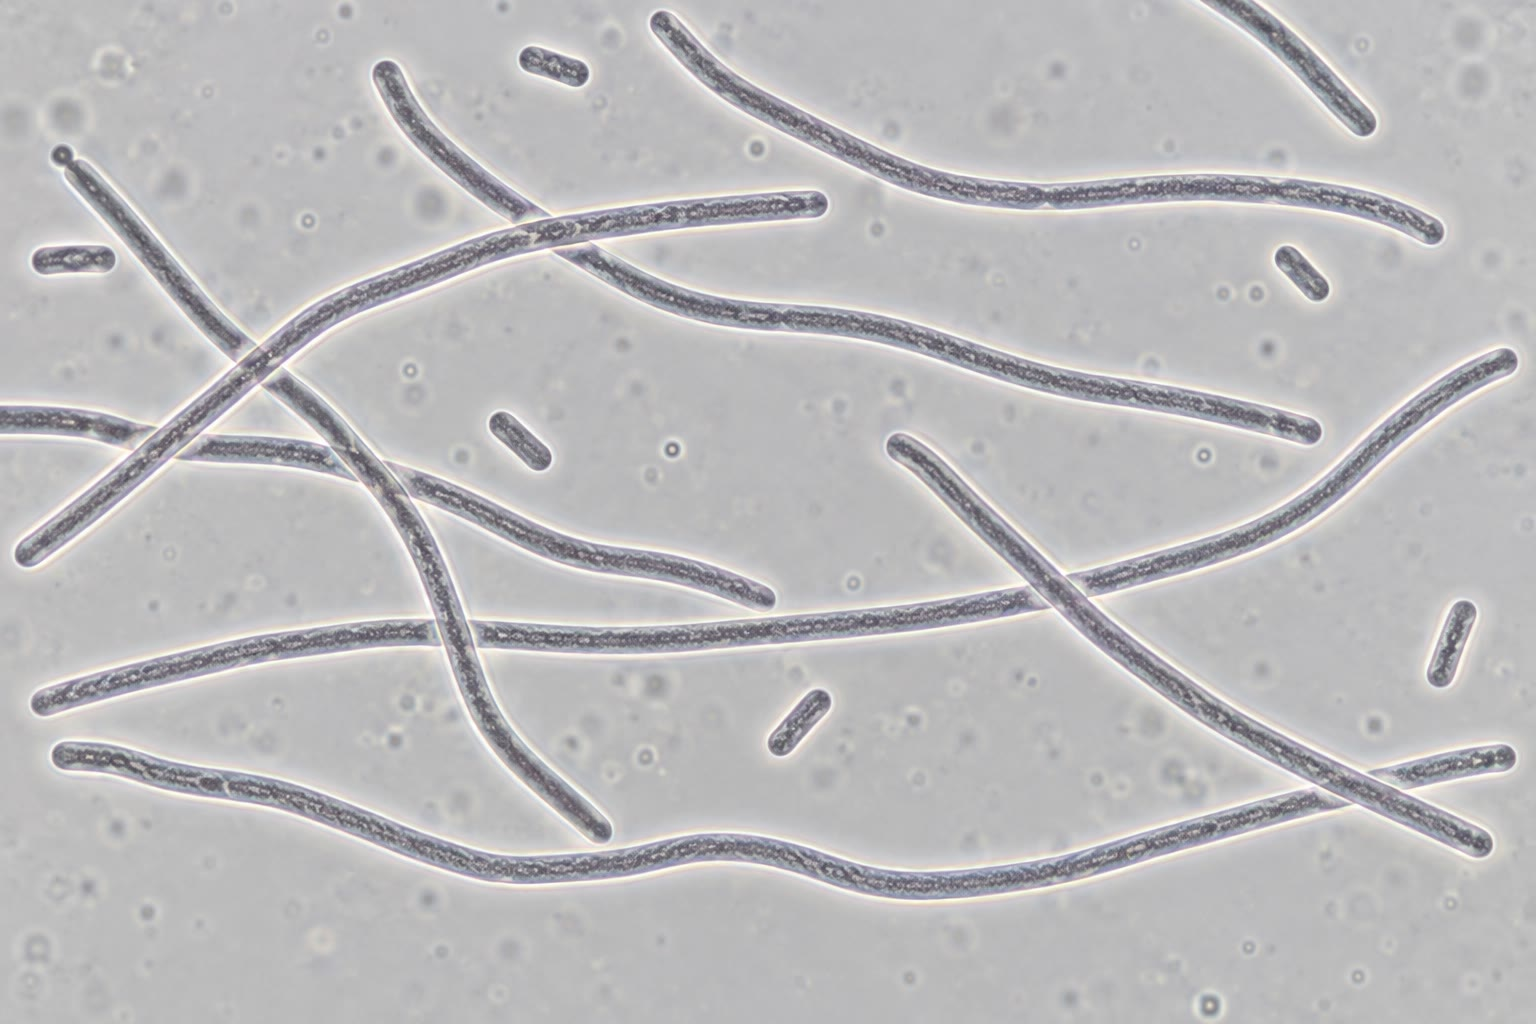
\includegraphics[width=0.46\linewidth]{images/book5/ai/b5-03-sos-filaments.jpg}\hspace{0.04\linewidth}
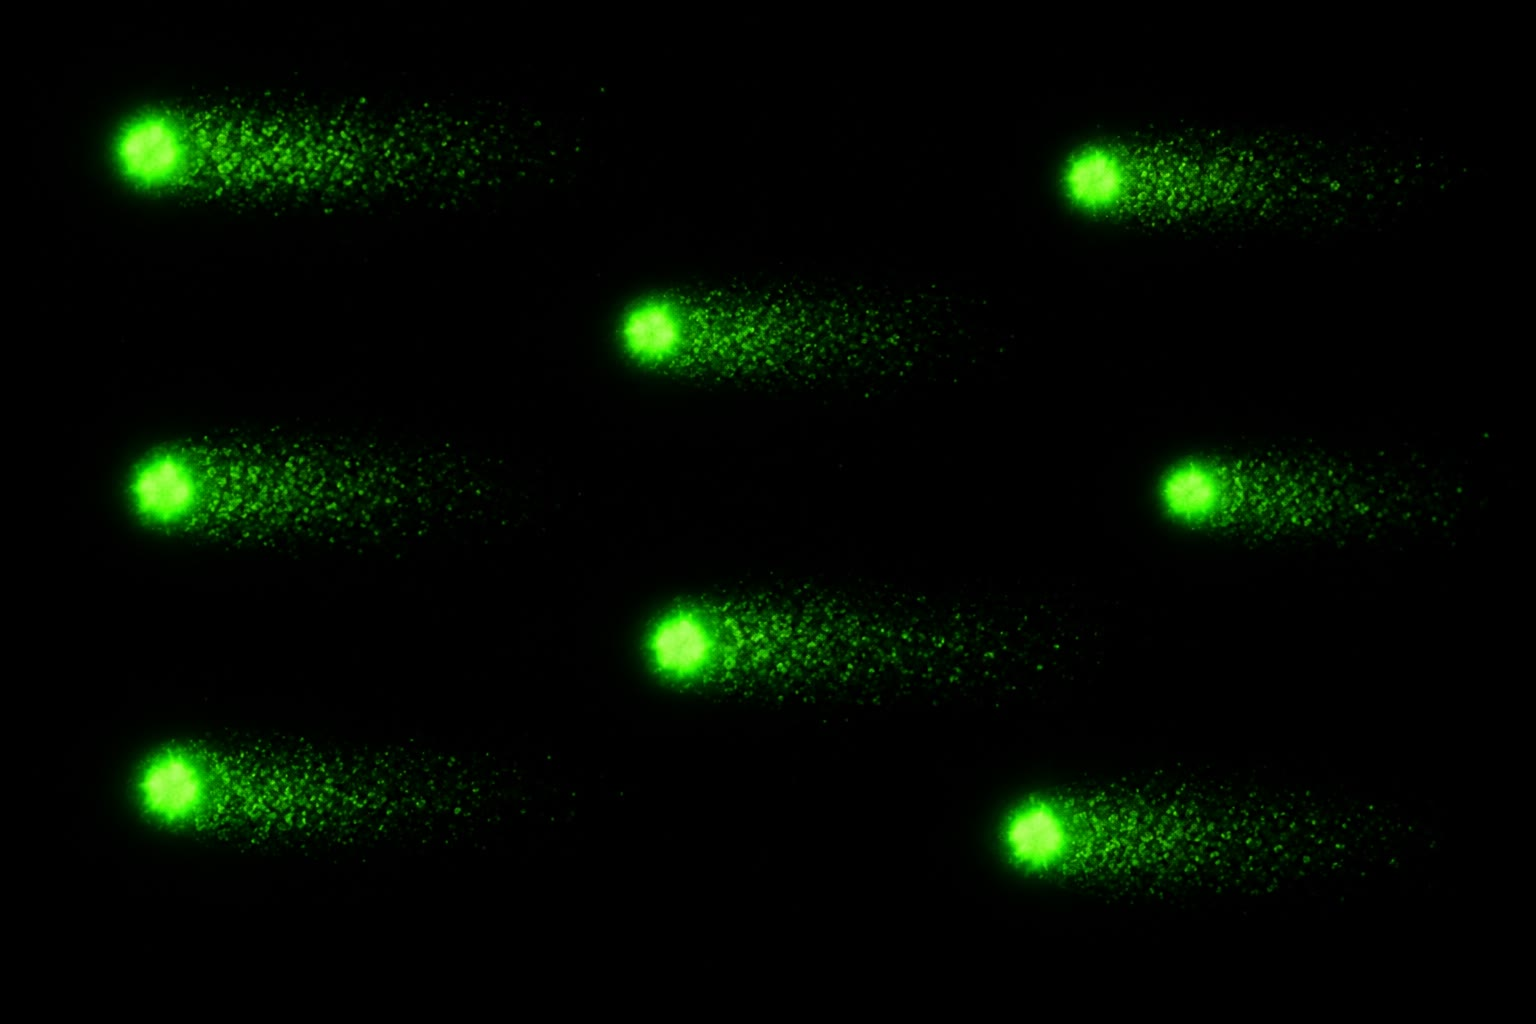
\includegraphics[width=0.46\linewidth]{images/book5/ai/b5-03-comet-assay.jpg}

{\small À gauche~: \emph{E.~coli} après irradiation ultraviolette,
allongée en longs filaments parce que la \omterm{prop:b3:dna-repair:sos}{réponse SOS} a bloqué la
division cellulaire pendant la réparation de l'ADN. À droite~: un essai
des comètes --- des cellules isolées enrobées dans un gel et soumises à
une électrophorèse~; l'ADN fragmenté sort du noyau en une traîne dont
la longueur mesure le nombre de cassures.}
\end{omfigure}

\begin{definition}[La réponse aux dommages de l'ADN]\label{def:b3:dna-repair:ddr}
\index{réponse aux dommages de l'ADN}\index{ATM}\index{point de contrôle}\index{p53}\index{gamma-H2AX}
Les eucaryotes signalent les dégâts par deux kinases~: \emph{ATM},
recrutée par le complexe MRN sur les \omterm{def:b3:dna-repair:lesions}{cassures double brin}, et
\emph{ATR}, recrutée sur l'ADN simple brin des fourches bloquées. Elles
phosphorylent des centaines de cibles. En quelques minutes l'\omterm{def:b3:chromatin-epigenetics:nucleosome}{histone}
H2AX est phosphorylée (\emph{$\gamma$-H2AX}) sur des mégabases autour
de chaque cassure, formant un foyer qui recrute les protéines de
réparation et qu'on peut compter au microscope, un foyer par cassure.
Les kinases Chk1 et Chk2 arrêtent le cycle cellulaire --- les
\emph{points de contrôle} du \cref{ch:b3:cell-cycle-apoptosis} --- en
inactivant les phosphatases qui commanderaient l'entrée en S ou en M~;
et le facteur de transcription \emph{p53}, stabilisé par
phosphorylation, induit l'inhibiteur de kinases dépendantes des
cyclines p21 (arrêt durable en G1), des gènes de réparation et, si les
dégâts sont lourds ou persistent, les gènes apoptotiques qui tuent la
cellule. La réponse achète du temps pour la réparation et, quand la
réparation échoue, supprime la cellule plutôt que de la laisser se
diviser avec un génome cassé.
\end{definition}

\begin{omfigure}
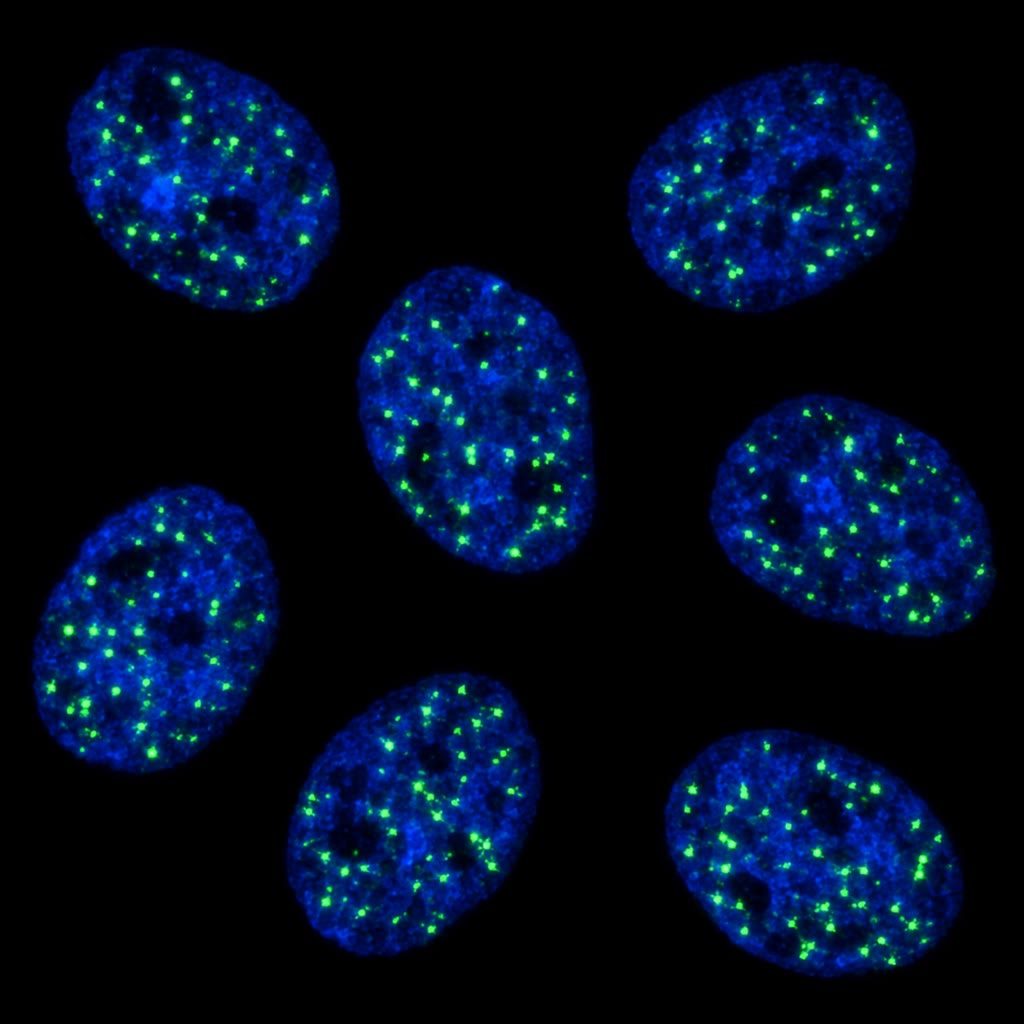
\includegraphics[width=0.4\linewidth]{images/book5/ai/b5-03-gamma-foci.jpg}

{\small Foyers de $\gamma$-H2AX (vert) dans des noyaux (bleu) une heure
après irradiation. Chaque foyer marque une \omterm{def:b3:dna-repair:lesions}{cassure double brin}~; les
compter mesure les dégâts et, dans les heures qui suivent, leur
réparation.}
\end{omfigure}

\begin{example}[Létalité synthétique~: BRCA et PARP]\label{ex:b3:dna-repair:parp}
Les femmes qui héritent d'une copie défectueuse de \emph{BRCA1} ou de
\emph{BRCA2} ont un risque de cancer du sein au cours de la vie de
\qtyrange{50}{80}{\%}~; les tumeurs naissent de cellules qui ont perdu
la seconde copie et ne savent plus faire de \omterm{def:b3:dna-repair:dsb}{recombinaison homologue}.
Ces cellules réparent leurs \omterm{def:b3:dna-repair:lesions}{cassures double brin} par la seule jonction
d'extrémités et accumulent des remaniements. Elles acquièrent aussi une
faiblesse précise. Les cassures simple brin, quelque \num{10000} par
jour, sont réparées par une voie qui a besoin de l'enzyme PARP~; quand
un médicament inhibe PARP, les cassures simple brin persistent jusqu'en
phase~S, où une fourche transforme chacune en une \omterm{def:b3:dna-repair:lesions}{cassure double brin} à
une seule extrémité --- réparable par la seule recombinaison. Une
cellule normale, avec un bon allèle \emph{\omterm{def:b3:dna-repair:dsb}{BRCA}}, s'en tire~; la cellule
tumorale meurt. Deux défauts, inoffensifs séparément, sont mortels
ensemble~: le médicament tue par \emph{létalité synthétique}, et
épargne les autres cellules de la patiente.
\end{example}

\begin{proposition}[La recombinaison comme outil]\label{prop:b3:dna-repair:tools}
\index{recombinaison site-spécifique}\index{Cre-lox}
Les recombinases site-spécifiques coupent et rejoignent l'ADN à de
courtes séquences définies, sans recherche d'homologie ni synthèse~:
l'enzyme Cre du phage P1 agit sur des sites \emph{loxP} de
\qty{34}{bp}, l'enzyme Flp de la levure sur des sites \emph{FRT}. Deux
sites de même orientation sur une même molécule excisent l'ADN qui les
sépare sous forme de cercle~; en orientations opposées ils l'inversent~;
des sites portés par deux molécules échangent leurs flancs. Un gène
encadré de sites \emph{loxP} («~floxé~») n'est supprimé que dans les
cellules où Cre est exprimée, depuis un promoteur au choix de
l'expérimentateur, ou au moment que celui-ci choisit si Cre n'est
rendue active que par un médicament~: c'est ainsi qu'on étudie dans le
foie adulte, ou dans le seul neurone, un gène indispensable à l'embryon
(\cref{ch:b3:genetic-engineering}). La \omterm{def:b3:dna-repair:dsb}{recombinaison homologue} propre à
la cellule est ce que le ciblage de gènes et l'édition dirigée par
CRISPR empruntent pour écrire une séquence choisie à un endroit choisi.
\end{proposition}

\begin{remark}[Réparation et vieillissement]\label{rem:b3:dna-repair:ageing}
Les cellules qui ne réparent pas accumulent des mutations, entrent en
sénescence ou meurent~; les défauts héréditaires de la réparation
(syndrome de Werner, une hélicase~; syndrome de Cockayne, réparation
couplée à la transcription~; ataxie-télangiectasie, \omterm{def:b3:dna-repair:ddr}{ATM}) donnent des
traits de vieillissement précoce, et le nombre de mutations somatiques
des tissus normaux croît linéairement avec l'âge, au rythme de
quelques dizaines de mutations par cellule et par an. Que les dégâts
accumulés \emph{causent} le vieillissement ordinaire, ou l'accompagnent
seulement, n'est pas tranché~; que la capacité de réparation détermine
en partie la longévité selon les espèces --- les espèces qui vivent
longtemps réparent davantage --- est bien établi.
\end{remark}

\section{Exercices}

\begin{exercise}[$\star$]\label{exo:b3:dna-repair:1}
Classer ces \omterm{def:b3:dna-repair:lesions}{lésions} en spontanées ou environnementales et nommer la
voie de réparation de chacune~: un uracile dans l'ADN~; un dimère de
thymines~; une \omterm{def:b3:dna-repair:lesions}{8-oxoguanine}~; un mésappariement G--T derrière la
fourche~; une \omterm{def:b3:dna-repair:lesions}{cassure double brin} en G1.
\end{exercise}

\begin{exercise}[$\star$]\label{exo:b3:dna-repair:2}
Pourquoi la \omterm{def:b3:dna-repair:excision}{réparation par excision de nucléotides} n'a-t-elle besoin
d'aucune enzyme propre à chaque type de \omterm{def:b3:dna-repair:lesions}{lésion}, alors que la \omterm{def:b3:dna-repair:excision}{réparation
par excision de base} a besoin d'une \omterm{def:b3:dna-repair:excision}{glycosylase} pour chacun~?
\end{exercise}

\begin{exercise}[$\star$]\label{exo:b3:dna-repair:3}
Énoncer le problème de discrimination des brins de la \omterm{prop:b3:dna-repair:fidelity}{réparation des
mésappariements} et la façon dont \emph{E.~coli} le résout. Que se
passerait-il chez un mutant \emph{dam}, qui ne méthyle aucun site GATC~?
\end{exercise}

\begin{exercise}[$\star$]\label{exo:b3:dna-repair:4}
Une cellule reçoit \qty{2}{Gy} de rayons X. Combien de \omterm{def:b3:dna-repair:lesions}{cassures double
brin} subit-elle, en gros, et combien de foyers de $\gamma$-H2AX
s'attendrait-on à compter une heure plus tard~? Pourquoi moins au bout
de six heures~?
\end{exercise}

\begin{exercise}[$\star\star$]\label{exo:b3:dna-repair:5}
À l'aide de la \cref{prop:b3:dna-repair:fidelity}, calculer le taux de
mutation par paire de bases et le nombre de mutations nouvelles par
génome diploïde et par division (a) dans une cellule normale, (b) dans
une cellule privée de \omterm{prop:b3:dna-repair:fidelity}{réparation des mésappariements}, (c) dans une
cellule dont la polymérase a perdu son exonucléase. Laquelle est la
mutatrice la plus dangereuse~?
\end{exercise}

\begin{exercise}[$\star\star$]\label{exo:b3:dna-repair:6}
Les sites abasiques apparaissent à raison de $10^{4}$ par cellule et
par jour et sont réparés avec une demi-vie de \qty{15}{min}. Utiliser
le \cref{thm:b3:dna-repair:load} pour trouver le nombre stationnaire de
sites abasiques dans une cellule. Si un médicament ralentit la
réparation d'un facteur dix, quel est le nouvel état stationnaire, et
combien de sites une fourche rencontrerait-elle si elle copie le génome
en \qty{8}{h}~?
\end{exercise}

\begin{exercise}[$\star\star$]\label{exo:b3:dna-repair:7}
En G2, une cassure peut être réparée par NHEJ (demi-vie \qty{30}{min})
ou par HR (demi-vie \qty{4}{h}), toutes deux disponibles. Quelle
fraction des cassures passe par la HR~? Quelle est la demi-vie des
cassures~? Pourquoi la HR est-elle malgré tout la voie qui compte aux
fourches de réplication effondrées~?
\end{exercise}

\begin{exercise}[$\star\star$]\label{exo:b3:dna-repair:8}
Prévoir le comportement des microsatellites, le spectre tumoral et la
sensibilité au soleil d'un patient atteint (a) du \omterm{def:b3:dna-repair:mmr}{syndrome de Lynch},
(b) d'un \omterm{def:b3:dna-repair:excision}{xeroderma pigmentosum} du groupe~A, (c) de la variante XP-V
dépourvue de Pol~$\eta$.
\end{exercise}

\begin{exercise}[$\star\star$]\label{exo:b3:dna-repair:9}
Deux sites \emph{loxP} de même orientation encadrent l'exon~3 d'un
gène~; Cre est exprimée depuis un promoteur actif seulement dans le
foie et dès la naissance. Décrire le génotype des cellules hépatiques
et des neurones chez l'adulte, et ce qui se passe si les sites sont
placés en orientations opposées.
\end{exercise}

\begin{exercise}[$\star\star\star$]\label{exo:b3:dna-repair:10}
Expliquer pourquoi la \omterm{prop:b3:dna-repair:sos}{réponse SOS} allume les gènes de réparation avant
les polymérases infidèles, en s'appuyant sur les affinités de LexA pour
leurs opérateurs, et pourquoi une bactérie totalement dépourvue de
polymérases infidèles pourrait malgré tout être désavantagée chez un
patient traité par antibiotiques.
\end{exercise}

\begin{exercise}[$\star\star\star$]\label{exo:b3:dna-repair:11}
Un inhibiteur de PARP tue les cellules tumorales déficientes en
\emph{\omterm{def:b3:dna-repair:dsb}{BRCA}} mais pas les cellules normales de la patiente. Exposer la
chaîne causale, puis prévoir deux façons dont une tumeur pourrait
devenir résistante au médicament et comment on détecterait chacune.
\end{exercise}

\begin{exercise}[$\star\star\star$]\label{exo:b3:dna-repair:12}
La conversion génique au voisinage d'un crossing-over donne des
tétrades $3{:}1$. Dessiner (ou décrire) une \omterm{def:b3:dna-repair:dsb}{jonction de Holliday} dont
l'hétéroduplex recouvre un marqueur, et montrer comment la \omterm{prop:b3:dna-repair:fidelity}{réparation
des mésappariements} de cet hétéroduplex donne $3{:}1$ dans un sens,
$1{:}3$ dans l'autre, et comment l'absence de réparation donne une
spore elle-même hétérozygote (une ségrégation post-méiotique). Pourquoi
la conversion est-elle cantonnée aux marqueurs voisins du
crossing-over~?
\end{exercise}

\section{Problème~: une journée dans la vie d'un génome}

\begin{problem}[{Problème du week-end --- les dégâts quotidiens d'une
cellule humaine dénombrés, l'échelle de fidélité multipliée, une dose
de soleil suivie jusqu'à la fourche dans une cellule normale et dans
une cellule déficiente, une dose de rayons X partagée entre deux voies
de réparation et la faiblesse d'une tumeur transformée en médicament,
pour finir sur le nombre de dimères que rencontre la fourche, le taux
de mutation par base et la fraction des cassures que répare la
recombinaison}]
\label{pb:b3:dna-repair:1}
Données~: une cellule humaine diploïde compte $6.4\times 10^{9}$ bp,
dont \qty{1.5}{\%} codantes. Dégâts spontanés par jour~: $10^{4}$
\omterm{def:b3:dna-repair:lesions}{dépurinations}, $400$ \omterm{def:b3:dna-repair:lesions}{désaminations} de cytosine, $10^{4}$ cassures
simple brin. Fidélité~: polymérase $10^{-5}$, la relecture laisse
$10^{-2}$ des erreurs, la \omterm{prop:b3:dna-repair:fidelity}{réparation des mésappariements} $10^{-3}$. Un
bain de soleil laisse $10^{5}$ \omterm{def:b3:dna-repair:lesions}{dimères de pyrimidines} par cellule
cutanée~; l'excision a une demi-vie de \qty{2}{h} normalement et de
\qty{70}{h} dans le \omterm{def:b3:dna-repair:excision}{xeroderma pigmentosum}~; une fourche arrive
\qty{8}{h} plus tard~; le contournement translésionnel d'un dimère
cause une mutation avec la probabilité $10^{-3}$. Les rayons X
produisent $35$ \omterm{def:b3:dna-repair:lesions}{cassures double brin} par gray~; demi-vie NHEJ
\qty{30}{min}, demi-vie HR \qty{4}{h}.

\medskip
\noindent\textbf{Partie I --- Les jours ordinaires.}
\begin{enumerate}
  \item Combien de \omterm{def:b3:dna-repair:lesions}{lésions} spontanées la cellule subit-elle par jour,
        et par an~? Comparer à la taille du génome.
  \item Calculer le taux de mutation par paire de bases et par
        division, et le nombre attendu de mutations nouvelles par
        division.
  \item Combien d'entre elles tombent en séquence codante~? Sur les
        quelque $50$ divisions qui séparent le zygote d'une cellule de
        peau adulte, combien de mutations codantes une cellule cutanée
        porte-t-elle du seul fait de la réplication~?
  \item Une cellule privée de \omterm{prop:b3:dna-repair:fidelity}{réparation des mésappariements}~: taux de
        mutation et mutations par division~? Un microsatellite glisse
        une fois sur $10^{4}$ divisions sans \omterm{prop:b3:dna-repair:fidelity}{réparation des
        mésappariements} et une fois sur $10^{7}$ avec elle. Dans une
        tumeur de $10^{9}$ cellules issue de $40$ divisions, combien de
        cellules portent un allèle glissé à un microsatellite donné
        dans chaque cas~? (Estimer par taux $\times$ divisions $\times$
        cellules.)
  \item La \omterm{def:b3:dna-repair:lesions}{désamination} de la cytosine donne un uracile, celle de la
        5-méthylcytosine une thymine. Laquelle est réparée, par quoi,
        et laquelle devient une mutation~? Faire le lien avec le
        déficit en \omterm{def:b3:chromatin-epigenetics:methylation}{CpG} du \cref{ch:b3:chromatin-epigenetics}.
  \item Une guanine oxydée (8-oxoG) s'apparie à A lors de la
        réplication. La cellule possède une \omterm{def:b3:dna-repair:excision}{glycosylase} pour la 8-oxoG
        en face d'un C, une autre pour l'A en face d'une 8-oxoG, et une
        hydrolase qui détruit le dGTP oxydé. Expliquer ce que chacune
        prévient et quelle mutation résulte de leur échec commun.
\end{enumerate}

\medskip
\noindent\textbf{Partie II --- Une journée au soleil.}
\begin{enumerate}[resume]
  \item Calculer les constantes d'excision $k$ pour la cellule normale
        et pour la cellule XP.
  \item Combien de dimères restent à l'arrivée de la fourche dans
        chacune~?
  \item Combien de mutations le bain de soleil cause-t-il par cellule
        dans chaque cas, et combien d'entre elles sont en séquence
        codante~?
  \item Au cours d'une enfance de $500$ expositions de ce genre,
        combien de mutations codantes par cellule cutanée dans chaque
        cas~? Comparer au nombre dû à la seule réplication de la
        question 3.
  \item Environ $20$ gènes, totalisant \qty{40}{kb} de séquence
        codante, peuvent déclencher un cancer cutané lorsqu'ils sont
        mutés. Quelle est la probabilité, par cellule, qu'au moins une
        mutation induite par le soleil tombe dans l'un d'eux, chez
        l'enfant XP~? (Utiliser une loi de Poisson de moyenne
        adéquate.) Avec $10^{9}$ cellules exposées, combien sont
        touchées~?
  \item Expliquer pourquoi le problème des cellules XP est un problème
        de la fourche et non de la \omterm{def:b3:dna-repair:lesions}{lésion} elle-même, et pourquoi les
        cancers n'apparaissent que sur la peau.
\end{enumerate}

\medskip
\noindent\textbf{Partie III --- Une dose de rayons X.}
\begin{enumerate}[resume]
  \item Une dose de \qty{2}{Gy}~: combien de \omterm{def:b3:dna-repair:lesions}{cassures double brin}, et
        combien de foyers de $\gamma$-H2AX au bout d'une heure si la
        NHEJ est la seule voie (cellule en G1)~?
  \item Dans une cellule en G2 les deux voies fonctionnent. Calculer
        les constantes de vitesse et la fraction des cassures réparées
        par la HR.
  \item Quelle est la demi-vie des cassures en G2, et combien en
        reste-t-il au bout d'une heure~?
  \item Chaque événement de NHEJ modifie quelques paires de bases à la
        jonction. Si une jonction tombe en séquence codante avec la
        probabilité $0.015$ et que la modification détruit alors le
        gène avec la probabilité $0.7$, combien de gènes la dose de
        \qty{2}{Gy} détruit-elle par cellule en G1~?
  \item Avec $n$ cassures simultanées, les extrémités peuvent être mal
        jointes en une translocation. Supposons que chacune des
        $n(n-1)/2$ paires de cassures soit jointe de travers avec la
        probabilité $3\times 10^{-4}$. Combien de translocations
        attendues par cellule à \qty{2}{Gy}~? Et à \qty{0.2}{Gy}~?
        Pourquoi le risque croît-il comme le carré de la dose alors que
        le nombre de cassures croît linéairement~?
  \item La même dose de \qty{2}{Gy} donnée en \qty{10}{h} au lieu d'un
        éclair~: combien de cassures sont présentes à un instant donné
        (état stationnaire, NHEJ)~? Qu'est-ce que cela implique pour
        les translocations, et pour la pratique du fractionnement en
        radiothérapie~?
  \item Une cellule survit à une dose $D$ avec la probabilité
        $e^{-D/D_{0}}$, avec $D_{0} = \qty{1.5}{Gy}$ pour une cellule à
        réparation intacte et \qty{0.5}{Gy} pour une cellule dépourvue
        de NHEJ. Calculer la survie de chacune à \qty{2}{Gy} et à
        \qty{6}{Gy}, et interpréter $D_{0}$.
\end{enumerate}

\medskip
\noindent\textbf{Partie IV --- La faiblesse de la tumeur.}
\begin{enumerate}[resume]
  \item Une cellule tumorale déficiente en \emph{BRCA2} ne répare ses
        cassures que par NHEJ. À l'aide de la question 14, quelle
        fraction de ses cassures de S/G2 est désormais réparée de façon
        infidèle là où une cellule normale l'aurait réparée fidèlement~?
        Qu'est-ce que cela fait à son génome au fil des années~?
  \item L'inhibition de PARP laisse non réparées les $10^{4}$ cassures
        simple brin quotidiennes~; \qty{1}{\%} d'entre elles sont
        converties en \omterm{def:b3:dna-repair:lesions}{cassures double brin} à une seule extrémité par
        les fourches. Combien de telles cassures par jour et par
        cellule, et pourquoi la NHEJ ne peut-elle pas réparer
        correctement une cassure à une seule extrémité~?
  \item Expliquer pourquoi les cellules normales de la patiente,
        hétérozygotes pour \emph{BRCA2}, survivent au médicament.
  \item Une tumeur devient résistante grâce à une seconde mutation qui
        rétablit le cadre de lecture de \emph{BRCA2}. Expliquer, et
        dire comment on le détecterait.
  \item Une chimiothérapie par un agent alkylant tue les cellules
        tumorales par l'intermédiaire de la \omterm{prop:b3:dna-repair:fidelity}{réparation des
        mésappariements}~: l'enzyme tente de réparer les bases alkylées
        et déclenche la mort cellulaire. Prévoir l'effet du médicament
        sur une tumeur de \omterm{def:b3:dna-repair:mmr}{syndrome de Lynch}, qui en est dépourvue.
  \item Énoncer les trois résultats~: les dimères rencontrés par la
        fourche dans la cellule XP (question~8), le taux de mutation
        normal par paire de bases (question~2) et la fraction des
        cassures de G2 que répare la HR (question~14).
\end{enumerate}
\end{problem}
